\input{../preamble-tmp.tex}

\title%
{Sockets TCP/IP en C++ - Redes TCP/IP}


\subject{Sockets TCP/IP en C++ - Redes TCP/IP}


\begin{document}

\begin{frame}[noframenumbering,plain]
   \titlepage
\end{frame}

~% macro content() %~
\section{Redes TCP/IP (simplificado)}

%   \begin{frame}[fragile]{Medios compartidos (simplificado)}
%      \begin{columns}
%          \begin{column}{.4\linewidth}
%              \begin{tikzpicture}[remember picture,overlay]
%                  \node[anchor=west] {
%                      ~% if interactive is off %~
%                      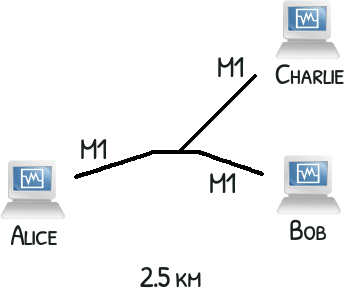
\includegraphics[width=.98\linewidth]{imgs/shared.png}
%                      ~% else %~
%                      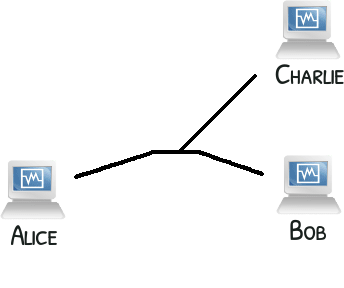
\includegraphics[width=.98\linewidth]{imgs/shared-incomplete.png}
%                      ~% endif %~
%                  };
%              \end{tikzpicture}
%          \end{column}
%         \begin{column}{.6\linewidth}
%           \begin{itemize}
%               \item<1-> Los mensajes son recibidos por todos (\textit{shared}).
%               \item<2-> No se requiere hardware adicional en la red.
%               \item<3-> Solo un participante puede hablar a la vez:\\
%                         La performance se degrada a mayor cantidad de participantes.
%           \end{itemize}
%         \end{column}
%      \end{columns}
%   \end{frame}
%   \note[itemize] {
%   \item Dado que el medio es compartido, cuando Alice envia un mensaje este se propaga por toda la red.
%   \item El mensaje es recibido entonces por todos los participantes.
%   \item Y a la vez evita que otros puedan comunicarse por que el medio esta en uso. Esto se conoce como \textit{half duplex}.
%   \item Este tipo de redes requieren un hardware adicional m\'inimo o nulo lo que las hace particularmente baratas y f\'aciles de mantener.
%   \item Son para redes locales, como una red Wifi.
%   }

\begin{frame}[fragile]{Internet - Protocolo IP (simplificado)}
   \begin{columns}
       \begin{column}{.4\linewidth}
           \begin{tikzpicture}[remember picture,overlay]
               \node[anchor=west] {
                   ~% if interactive is off %~
                   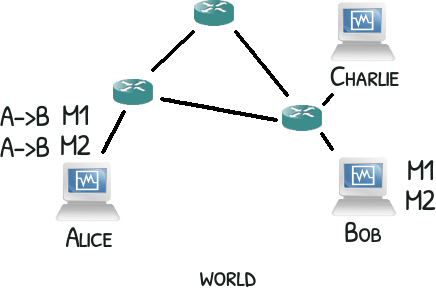
\includegraphics[width=.98\linewidth]{imgs/internet.png}
                   ~% else %~
                   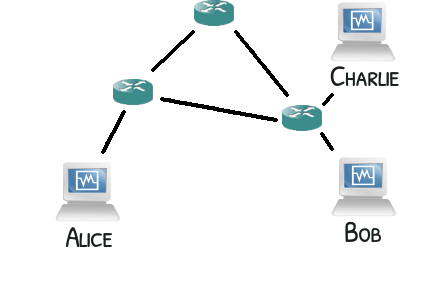
\includegraphics[width=.98\linewidth]{imgs/internet-incomplete.png}
                   ~% endif %~
               };
           \end{tikzpicture}
       \end{column}
      \begin{column}{.6\linewidth}
        \begin{itemize}
            \item<1-> Los mensajes son \textit{ruteados} a sus destinos (\textit{hosts})
            \item<2-> Dos esquemas de direcciones: IPv4 (4 bytes) e IPv6 (16 bytes).
            \item<3-> Son redes \textit{best effort}
            \only<3> {
            \begin{itemize}
                \item Los paquetes se pueden perder.
                \item Los paquetes puede llegar en desorden.
                \item Los paquetes puede llegar duplicados.
            \end{itemize}
            }
        \end{itemize}
      \end{column}
   \end{columns}
\end{frame}
\note[itemize] {
\item Ahora la red esta segmentada: los mensajes son enviados de un segmento a otro a traves de los routers.
\item Los routers usan las direcciones IP de destino para saber a donde enviar los mensajes.
\item La red esta governada por el protocolo IP. Existen actualmente 2 versiones IPv4 e IPv6.
\item El primero usa direcciones de m\'aquina (host) de 4 bytes y el segundo de 16.
\item IP no garantiza que lleguen todos los paquetes, ni el orden ni que no haya duplicados.
\item Es un protocolo pensado para simplificar el hardware de la red, no para hacerle m\'as f\'acil la vida a los desarrolladores.
}

\begin{frame}[fragile]{Internet - Protocolo TCP (simplificado)}
   \begin{columns}
       \begin{column}{.4\linewidth}
           \begin{tikzpicture}[remember picture,overlay]
               \node[anchor=west] {
                   ~% if interactive is off %~
                   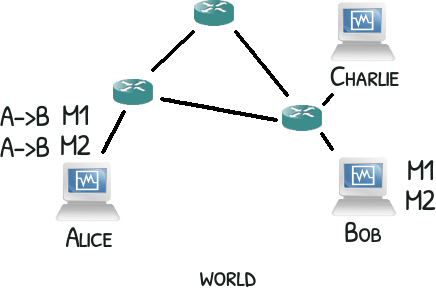
\includegraphics[width=.98\linewidth]{imgs/internet.png}
                   ~% else %~
                   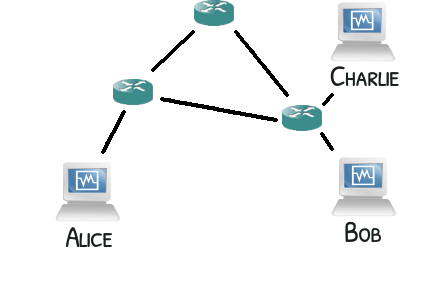
\includegraphics[width=.98\linewidth]{imgs/internet-incomplete.png}
                   ~% endif %~
               };
           \end{tikzpicture}
       \end{column}
      \begin{column}{.6\linewidth}
        \begin{itemize}
            \item<1-> Corre sobre IP, permite el direccionamiento a nivel de servicio (\textit{port})
            \item<2-> Orientado a bytes, no a mensajes (\textit{stream}): los bytes no se pierden, desordenan ni duplican \alert{pero no garantiza \textit{boundaries}}
            \item<3-> Con conexi\'on y full-duplex. \alert{An\'alogo a un archivo binario secuencial.}
        \end{itemize}
      \end{column}
   \end{columns}
\end{frame}
\note[itemize] {
\item IP solo nos habla de los hosts, no de los programas que corren en ellos.
\item TCP permite direccionar a cada programa o servicio a traves de un n\'umero, el puerto.
\item TCP es orientado a la conexi\'on: hay un participante pasivo que espera una comunicaci\'on y hay otro que la inicia de forma activa.
\item T\'ipicamente el participante pasivo es el servidor y el activo el cliente.
\item Una vez establecida la conexi\'on los bytes enviados (full duplex) no se pierden, desordenan ni duplican.
\item TCP no garantiza nada sobre los mensajes, solo sabe de bytes, por lo que un mensaje puede llegar incompleto.
}

%   \begin{frame}[fragile]{Internet - Protocolo DNS (simplificado)}
%      \begin{columns}
%          \begin{column}{.4\linewidth}
%              \begin{tikzpicture}[remember picture,overlay]
%                  \node[anchor=west] {
%                      ~% if interactive is off %~
%                      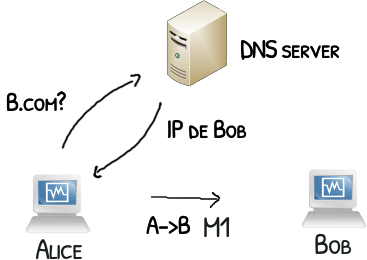
\includegraphics[width=.98\linewidth]{imgs/dns.png}
%                      ~% else %~
%                      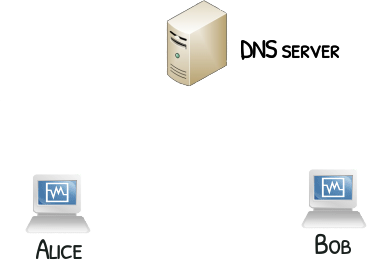
\includegraphics[width=.98\linewidth]{imgs/dns-incomplete.png}
%                      ~% endif %~
%                  };
%              \end{tikzpicture}
%          \end{column}
%         \begin{column}{.6\linewidth}
%           \begin{itemize}
%               \item<1-> No es necesario recordar la direcci\'on IP del destino (4 o 16 bytes) sino su \textit{nombre de dominio}.
%               \item<2-> La registraci\'on de dominios se hace a nivel gubernamental. Para el caso \lstinline[style=normal]!.com.ar! lo hace NIC, Canciller\'ia Argentina.
%               \item<3-> La resoluci\'on de un dominio a una o varias direcciones IP las hace el servidor de DNS.
%               \item<4-> Un dominio puede tener m\'ultiples IPs: por redundancia o por ser IPv4 e IPv6.
%           \end{itemize}
%         \end{column}
%      \end{columns}
%   \end{frame}

~% endmacro %~

~{ content() }~

\end{document}
